%========================================================
\chapter{Machine Learning Theory}
\label{chap:ml_theory}
%========================================================

This chapter forms the second theoretical pillar of this thesis, introducing the machine learning concepts used to model the interest rate term structures established in the first. We cover feedforward neural networks, encoder--decoder architectures and the procedures used to train such models.



%--------------------------------------------------------
\section{Neural Networks}
\label{sec:neural_networks}
%--------------------------------------------------------


A neural network is built from neurons and layers, with the full network obtained by composing layers, as illustrated in Figure \ref{fig:nn_general}. We introduce each in turn.

\begin{figure}[H]
\centering
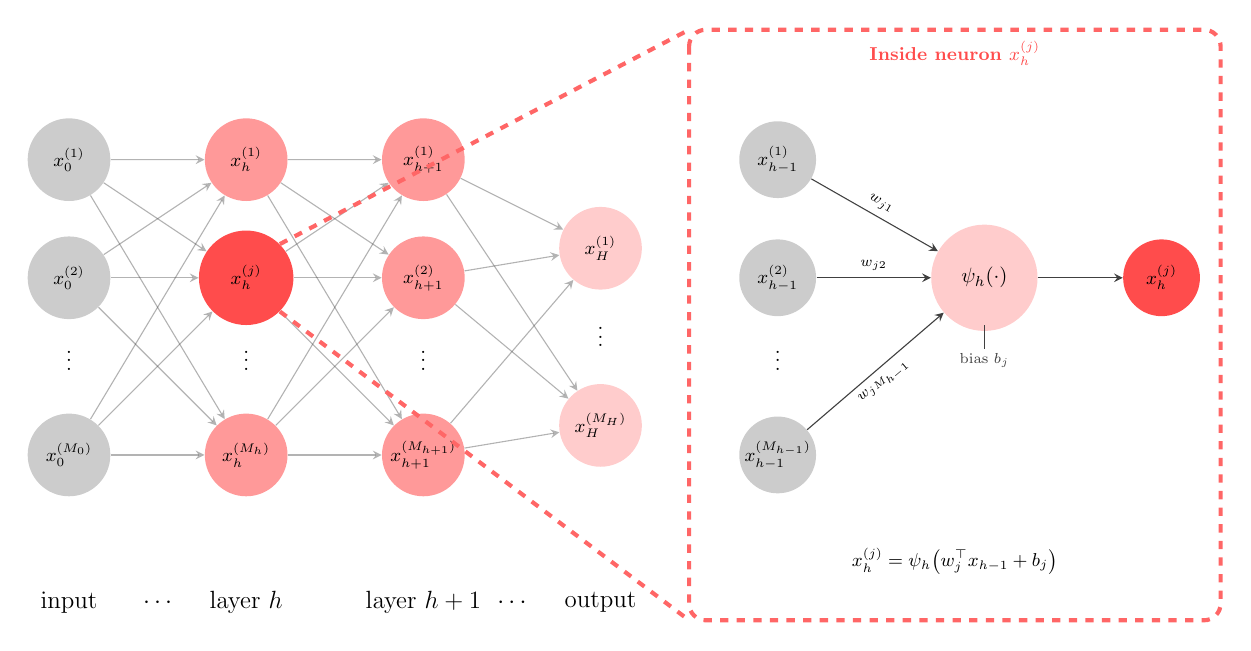
\begin{tikzpicture}[
    scale=0.75,
    transform shape,
    neuron/.style={circle, minimum size=14mm, inner sep=0pt},
    >=stealth
]
\definecolor{darkgrey}{RGB}{90,90,90}

% ======================
% Input layer (h=0)
% ======================
\node[neuron, fill=gray!40] (X01) at (0,  3.0) {\small$x_0^{(1)}$};
\node[neuron, fill=gray!40] (X02) at (0,  1.0) {\small$x_0^{(2)}$};
\node at (0, -0.3) {$\vdots$};
\node[neuron, fill=gray!40] (X0M) at (0, -2.0) {\small$x_0^{(M_0)}$};

% ======================
% Hidden layer h
% ======================
\node[neuron, fill=red!40] (Xh1) at (3,  3.0) {\small$x_h^{(1)}$};
\node[neuron, fill=red!70, minimum size=16mm] (Xhj) at (3,  1.0) {\small$x_h^{(j)}$};
\node at (3, -0.3) {$\vdots$};
\node[neuron, fill=red!40] (XhM) at (3, -2.0) {\small$x_h^{(M_h)}$};

% ======================
% Hidden layer h+1
% ======================
\node[neuron, fill=red!40] (Xh11) at (6,  3.0) {\small$x_{h+1}^{(1)}$};
\node[neuron, fill=red!40] (Xh12) at (6,  1.0) {\small$x_{h+1}^{(2)}$};
\node at (6, -0.3) {$\vdots$};
\node[neuron, fill=red!40] (Xh1M) at (6, -2.0) {\small$x_{h+1}^{(M_{h+1})}$};

% ======================
% Output layer H
% ======================
\node[neuron, fill=red!20] (XH1) at (9,  1.5) {\small$x_H^{(1)}$};
\node at (9,  0.1) {$\vdots$};
\node[neuron, fill=red!20] (XHM) at (9, -1.5) {\small$x_H^{(M_H)}$};

% ======================
% Connections
% ======================
\foreach \s in {X01,X02,X0M} {
    \foreach \t in {Xh1,Xhj,XhM} {
        \draw[->, draw=darkgray, opacity=0.4] (\s) -- (\t);
    }
}
\foreach \s in {Xh1,Xhj,XhM} {
    \foreach \t in {Xh11,Xh12,Xh1M} {
        \draw[->, draw=darkgray, opacity=0.4] (\s) -- (\t);
    }
}
\foreach \s in {Xh11,Xh12,Xh1M} {
    \foreach \t in {XH1,XHM} {
        \draw[->, draw=darkgray, opacity=0.4] (\s) -- (\t);
    }
}

% ======================
% Layer labels
% ======================
\large
\node at (0,  -4.5) {input};
\node at (1.5,-4.5) {$\cdots$};
\node at (3,  -4.5) {layer $h$};
\node at (6,  -4.5) {layer $h+1$};
\node at (7.5,-4.5) {$\cdots$};
\node at (9,  -4.5) {output};
\normalsize

% ======================
% Detail box
% ======================
\draw[dashed, red!60, rounded corners=6pt, line width=1.5pt]
    (10.5, 5.2) rectangle (19.5, -4.8);
\node[red!70, font=\small\bfseries] at (15.0, 4.8)
    {Inside neuron $x_h^{(j)}$};

% Leader lines from Xhj to detail box
\draw[dashed, red!60, line width=1.5pt] (Xhj.north east) -- (10.5,  5.2);
\draw[dashed, red!60, line width=1.5pt] (Xhj.south east) -- (10.5, -4.8);

% Mini input nodes inside detail box
\node[neuron, fill=gray!40, minimum size=13mm] (CX1) at (12.0,  3.0) {\small$x_{h-1}^{(1)}$};
\node[neuron, fill=gray!40, minimum size=13mm] (CX2) at (12.0,  1.0) {\small$x_{h-1}^{(2)}$};
\node at (12.0, -0.3) {$\vdots$};
\node[neuron, fill=gray!40, minimum size=13mm] (CXM) at (12.0, -2.0) {\small$x_{h-1}^{(M_{h-1})}$};

% Central neuron in detail box
\node[neuron, fill=red!20, minimum size=18mm] (CN) at (15.5, 1.0) {$\psi_h(\cdot)$};

% Output node in detail box
\node[neuron, fill=red!70, minimum size=13mm, font=\small, inner sep=1pt] (CO) at (18.5, 1.0) {$x_h^{(j)}$};

% Weighted arrows inside detail box
\draw[->, draw=darkgray] (CX1) -- node[above, sloped, font=\scriptsize] {$w_{j1}$} (CN);
\draw[->, draw=darkgray] (CX2) -- node[above, font=\scriptsize]         {$w_{j2}$} (CN);
\draw[->, draw=darkgray] (CXM) -- node[below, sloped, font=\scriptsize] {$w_{jM_{h-1}}$} (CN);
\draw[->, draw=darkgray] (CN)  -- (CO);

% Bias annotation
\node[font=\scriptsize, darkgray] at (15.5, -0.4) {bias $b_j$};
\draw[darkgray, thin] (15.5, -0.2) -- (15.5, 0.2);

% Equation inside detail box
\node[font=\small] at (15.0, -3.8)
    {$x_h^{(j)} = \psi_h\!\left(w_j^\top x_{h-1} + b_j\right)$};

\end{tikzpicture}
\caption{General feedforward network of depth $H$. Each node $x_h^{(j)}$
denotes the $j$-th neuron in layer $h$, for $j = 1,\ldots,M_h$.
The detail panel shows how neuron $x_h^{(j)}$ computes its output from the
previous layer $x_{h-1}$ via weights $w_j$, bias $b_j$, and
activation function $\psi_h$.}
\label{fig:nn_general}
\end{figure}



\begin{description}
    \item[Neurons]
A \emph{neuron} is a map from a vector $x \in \mathbb{R}^n$ to a scalar $\mathcal{N}(x)\in \mathbb{R}$:
\begin{equation}
    \mathcal{N}(x)
    = \psi(w^\top x + b),
    \qquad x \in \mathbb{R}^n,
\label{eq:neuron}
\end{equation}
where $w \in \mathbb{R}^n$ is a weight vector, $b \in \mathbb{R}$ is a bias, and $\psi : \mathbb{R} \to \mathbb{R}$ is an \emph{activation function}, with the computation illustrated in the detail panel of Figure \ref{fig:nn_general}. If $\psi$ is linear, the neuron reduces to an affine map, and a composition of affine maps remains affine. A network composed only of such neurons can only represent affine functions of the input. Choosing $\psi$ to be nonlinear allows networks to represent more complex input--output relationships. Common choices include the logistic sigmoid $\psi(t) = (1 + e^{-t})^{-1}$, the hyperbolic tangent $\psi(t) = \tanh(t)$, and the rectified linear unit $\psi(t) = \max(0,t)$.
    
    \item[Layers]
A \emph{layer} consists of neurons operating in parallel on the same input vector, each with its own weights and bias, as shown in Figure \ref{fig:nn_general}. We index the layers by $h = 1,\dotsc,H$, where different layers may have different numbers of neurons $M_h$. The number of neurons in layer $h$ is referred to as the \emph{width} of that layer. The outputs of all neurons in the layer are stacked into a vector, which becomes the input to the next layer. Explicitly, a layer computes
\begin{equation}
    x_h = \psi_h(W_h x_{h-1} + b_h),
\label{eq:layer}
\end{equation}
where $x_{h-1} \in \mathbb{R}^{M_{h-1}}$ denotes the output of the preceding layer, $W_h \in \mathbb{R}^{M_h \times M_{h-1}}$ is the weight matrix whose $i$th row contains the weights of the $i$th neuron, and $b_h \in \mathbb{R}^{M_h}$ is the bias vector. The activation function $\psi_h$ is applied element-wise.

    \item[Networks]
A \emph{network} is formed by composing $H$ layers in sequence \citep[Ch.~6]{Goodfellow2016}. Let $x = x_0 \in \mathbb{R}^{M_0}$ denote the input. Applying \eqref{eq:layer} successively through the $H$ layers yields the network output $x_H \in \mathbb{R}^{M_H}$. The final layer is referred to as the \emph{output layer}, while the preceding layers are called \emph{hidden layers} since their outputs $x_1,\ldots,x_{H-1}$ are internal to the network. The full network therefore represents the composition
\begin{equation}
    f(x;\Omega)
    = \psi_H\!\bigl(W_H\,\psi_{H-1}(\cdots
      \psi_1(W_1 x + b_1)\cdots) + b_H\bigr),
\label{eq:network}
\end{equation}
with parameter set $\Omega = \{W_h, b_h\}_{h=1}^H$. The number of layers $H$ is called the \emph{depth} of the network.
\end{description}


Networks that process information in one direction, from input to output, with no connections feeding back to earlier layers, are called \emph{feedforward} neural networks or \emph{multilayer perceptrons}. The network introduced above is of this type, and is the class considered throughout this thesis.


\section{Neural Networks as Function Approximators}

The goal is to find parameters $\Omega$ such that the neural network $f(x;\Omega)$ approximates some target function $f^*$ well. Each parameter set $\Omega = \{W_h, b_h\}_{h=1}^H$ determines a function, and the full set of functions representable by the network is the class
\[
    \bigl\{f(\,\cdot\,;\Omega) : \Omega \in \Theta\bigr\},
\]
where $\Theta\subseteq\mathbb{R}^p$ denotes the parameter space and $p$ is the total number of parameters. How suitable parameters are found is addressed in Section \ref{sec:training}. A natural question is whether this class is rich enough to approximate continuous target functions on compact domains. The following classical universal approximation result provides such a guarantee.

\begin{theorem}[Finite-dimensional universal approximation theorem, cf.\ \citealt{Leshno1993}]
\label{thm:UAT}
Let $\psi : \mathbb{R} \to \mathbb{R}$ be continuous and non-polynomial. Then for any compact set $K \subset \mathbb{R}^{M_0}$, any continuous target function $f^* : K \to \mathbb{R}$, and any $\varepsilon > 0$, there exist a width $M_1 \in \mathbb{N}$ and parameters
\[
    \Omega = (W_1,b_1,W_2,b_2),
\]
with
\[
    W_1 \in \mathbb{R}^{M_1 \times M_0},
    \qquad
    b_1 \in \mathbb{R}^{M_1},
    \qquad
    W_2 \in \mathbb{R}^{1 \times M_1},
    \qquad
    b_2 \in \mathbb{R},
\]
such that the network
\[
    f(x;\Omega) = W_2\,\psi(W_1x+b_1) + b_2,
\]
where $\psi$ is applied element-wise, satisfies
\[
    \sup_{x \in K} |f^*(x)-f(x;\Omega)| < \varepsilon.
\]
\end{theorem}

The approximating function in Theorem~\ref{thm:UAT} is a feedforward network with a single hidden layer of width $M_1$ and an identity activation in the output layer, and is therefore a special case of the general architecture in \eqref{eq:network}. The theorem, however, is an existence result only. It does not specify how large the width $M_1$ must be, nor whether deeper architectures can achieve the same approximation more efficiently. 

%--------------------------------------------------------
\section{Encoder--Decoder Architectures}
\label{sec:encoder_decoder}
%--------------------------------------------------------

An encoder--decoder architecture is a neural network consisting of two components:

\begin{description}
    \item[Encoder]
    The encoder $E$ maps an input $x$ to a latent representation $z = E(x)$.

    \item[Decoder]
    The decoder $D$ maps the latent representation to an output $y = D(z)$.
\end{description}

When the input and output domains coincide and the objective is to reconstruct the input, the architecture is referred to as an \emph{autoencoder} \citep[Ch.~14]{Goodfellow2016}. For an input $x \in \mathbb{R}^d$, the model takes the form
\[
    x \xrightarrow{\;E\;} z \xrightarrow{\;D\;} \hat{x},
\]
where $\hat{x}$ denotes the reconstruction of $x$.

If the latent dimension is smaller than the input dimension, $z \in \mathbb{R}^k$ with $k < d$, the autoencoder is called \emph{undercomplete} \citep[Ch.~14]{Goodfellow2016}. The latent representation is then more compact than the input, forcing the network to represent the input through a lower-dimensional bottleneck. When trained to achieve accurate reconstruction, the latent vector $z$ may therefore be interpreted as a compressed representation of $x$, useful for dimensionality reduction. 





\section{Training}
\label{sec:training}

Training a neural network amounts to finding the parameter set $\Omega$ that minimises the empirical risk
\begin{equation}
    \mathcal{L}(\Omega) = \frac{1}{N}\sum_{n=1}^{N} \ell\bigl(y_n,\, f(x_n;\Omega)\bigr),
\label{eq:empirical_risk}
\end{equation}
where $\mathcal{D} = \{(x_n, y_n)\}_{n=1}^N$ is the training dataset of $N$ observations, $f(x_n;\Omega)$ is the predicted output, and $\ell$ is a loss function measuring the discrepancy between target and prediction. Since the target and predicted outputs are vectors, a natural choice is the squared Euclidean norm
\[
    \ell\bigl(y,\, f(x;\Omega)\bigr) = \|y - f(x;\Omega)\|^2,
\]
which sums the squared errors across all output components. In general, this problem does not admit a closed-form solution, and one therefore relies on iterative numerical methods. When $\mathcal{L}$ is differentiable with respect to $\Omega$, the gradient $\nabla_\Omega \mathcal{L}$ gives the direction of steepest ascent of the loss, and gradient-based methods can therefore be employed. Consequently, moving the parameters in the opposite direction decreases it \citep[Chs.~6,~8]{Goodfellow2016}. We next turn to the specific gradient-based methods.



\subsection{Gradient descent}

The basic parameter update rule is \emph{gradient descent}. At each iteration, the parameters are updated by taking a step in the direction of the negative gradient:
\begin{equation}
    \Omega_{k+1}
    =
    \Omega_k - \gamma \nabla_\Omega \mathcal{L}(\Omega_k),
\label{eq:gd}
\end{equation}
where $\gamma > 0$ is the \emph{learning rate}, controlling the step size \citep[Ch.~8]{Goodfellow2016}. If $\gamma$ is too large, the updates may overshoot and the loss may diverge; if it is too small, convergence is slow. The learning rate is therefore an important hyperparameter to set in practice.

\subsection{Stochastic gradient descent and mini-batches}

For large datasets $\mathcal{D}$, computing the full gradient of the empirical risk \eqref{eq:empirical_risk} at every iteration can be computationally expensive. Instead, one may approximate the gradient using only part of the dataset $\mathcal{D}$. Given a batch $\mathcal{B} \subset \mathcal{D}$ of size $B$, the corresponding gradient approximation is
\begin{equation}
    \nabla_\Omega \mathcal{L}_{\mathcal{B}}(\Omega)
    =
    \frac{1}{B}
    \sum_{(x_n,y_n)\in\mathcal{B}}
    \nabla_\Omega\,\ell\bigl(y_n,\, f(x_n;\Omega)\bigr).
\label{eq:minibatch_grad}
\end{equation}
If the batch is sampled uniformly at random, this provides an unbiased estimator of the full gradient. The case $B=1$ is referred to as \emph{stochastic gradient descent}, while the case $1 < B < N$ is called \emph{mini-batch stochastic gradient descent}. Mini-batch methods are commonly used when training neural networks, since they allow efficient computation while providing more stable updates than pure stochastic gradient descent \citep[Ch.~8]{Goodfellow2016}. One complete pass through the dataset is referred to as an \emph{epoch}.

\subsection{The Adam optimiser}
\label{subsec:adam}

A widely used variant of stochastic gradient descent is the Adam optimiser of \citet{Kingma2015}. Adam constructs parameter updates using running averages of both the gradient and its element-wise square. Denoting the stochastic gradient at iteration $k$ by
\[
    g_k = \nabla_\Omega \mathcal{L}_{\mathcal{B}}(\Omega_k),
\]
the first and second moment estimates are defined recursively by
\begin{align}
    m_k &= \beta_1 m_{k-1} + (1-\beta_1) g_k, \\
    v_k &= \beta_2 v_{k-1} + (1-\beta_2) g_k^2,
\end{align}
where $m_k$ estimates the mean of the gradient and $v_k$ estimates its uncentred second moment, with the square taken element-wise. The constants $\beta_1,\beta_2 \in (0,1)$ are user-specified hyperparameters that determine how strongly past gradients influence the current estimates.

Because these recursions are typically initialised at zero, Adam applies the bias corrections
\[
    \hat{m}_k = \frac{m_k}{1-\beta_1^k},
    \qquad
    \hat{v}_k = \frac{v_k}{1-\beta_2^k}.
\]
The parameter update is then given by
\begin{equation}
    \Omega_{k+1}
    =
    \Omega_k
    -
    \gamma_k\,
    \frac{\hat{m}_k}{\sqrt{\hat{v}_k}+\epsilon},
\label{eq:adam}
\end{equation}
where $\gamma_k > 0$ is the learning rate at iteration $k$ and $\epsilon > 0$ is a small constant included for numerical stability. Unlike mini-batch stochastic gradient descent, Adam does not base the update solely on the gradient from the current mini-batch. Instead, it incorporates information from recent gradients, accounting for both their average direction and their magnitude.

\subsection{Backpropagation}
\label{subsec:backprop}

The optimisation methods described above require gradients of the empirical risk with respect to the network parameters. These gradients are computed efficiently by the \emph{backpropagation algorithm}, which applies the chain rule backwards through the layers of the network \citep[Ch.~6]{Goodfellow2016}. When working with a mini-batch, the gradients are computed for each observation in the batch and then averaged. The mechanics are illustrated below for a single training example with one observation.


\begin{example}
Consider a scalar-input network with one hidden neuron and a linear output layer:
\[
    a_1 = w_1 x + b_1,
    \qquad
    x_1 = \psi(a_1),
    \qquad
    \hat{y} = w_2 x_1 + b_2.
\]
with squared-error loss
\[
    L = (y-\hat{y})^2,
\]
The forward pass computes $a_1$, $x_1$, $\hat{y}$ and $L$ in sequence. The derivative with respect to the first-layer weight $w_1$ is then obtained by applying the chain rule backwards through these intermediate quantities,
\[
    \frac{\partial L}{\partial w_1}
    =
    \frac{\partial L}{\partial \hat{y}}
    \frac{\partial \hat{y}}{\partial x_1}
    \frac{\partial x_1}{\partial a_1}
    \frac{\partial a_1}{\partial w_1}
    =
    2(\hat{y}-y)\, w_2\, \psi'(a_1)\, x,
\]
combining the local derivatives along the path through which $w_1$ affects $L$. \;\;$\circ$
\end{example}

A \emph{computational graph} records these calculation steps. For the derivative in the example above, the relevant path is
\[
    w_1
    \;\longrightarrow\;
    a_1
    \;\longrightarrow\;
    x_1
    \;\longrightarrow\;
    \hat{y}
    \;\longrightarrow\;
    L.
\]
The forward pass computes and stores the intermediate values along this path. The backward pass then starts from the loss and applies the chain rule in the opposite direction to compute the gradients with respect to the parameters.

In modern machine learning frameworks, this process is handled by
\emph{automatic differentiation}. The framework records the operations carried out in the forward pass and, once the loss has been computed, automatically applies backpropagation to calculate the gradients needed for optimisation.
